\documentclass[]{article}
\usepackage{hyperref}
\usepackage{graphicx}
\usepackage{fullpage}

\hyphenpenalty=100000
\DeclareGraphicsExtensions{.png}

\newcommand{\MT}{\textbf{MemoryTamer}}

\begin{document}

\title{
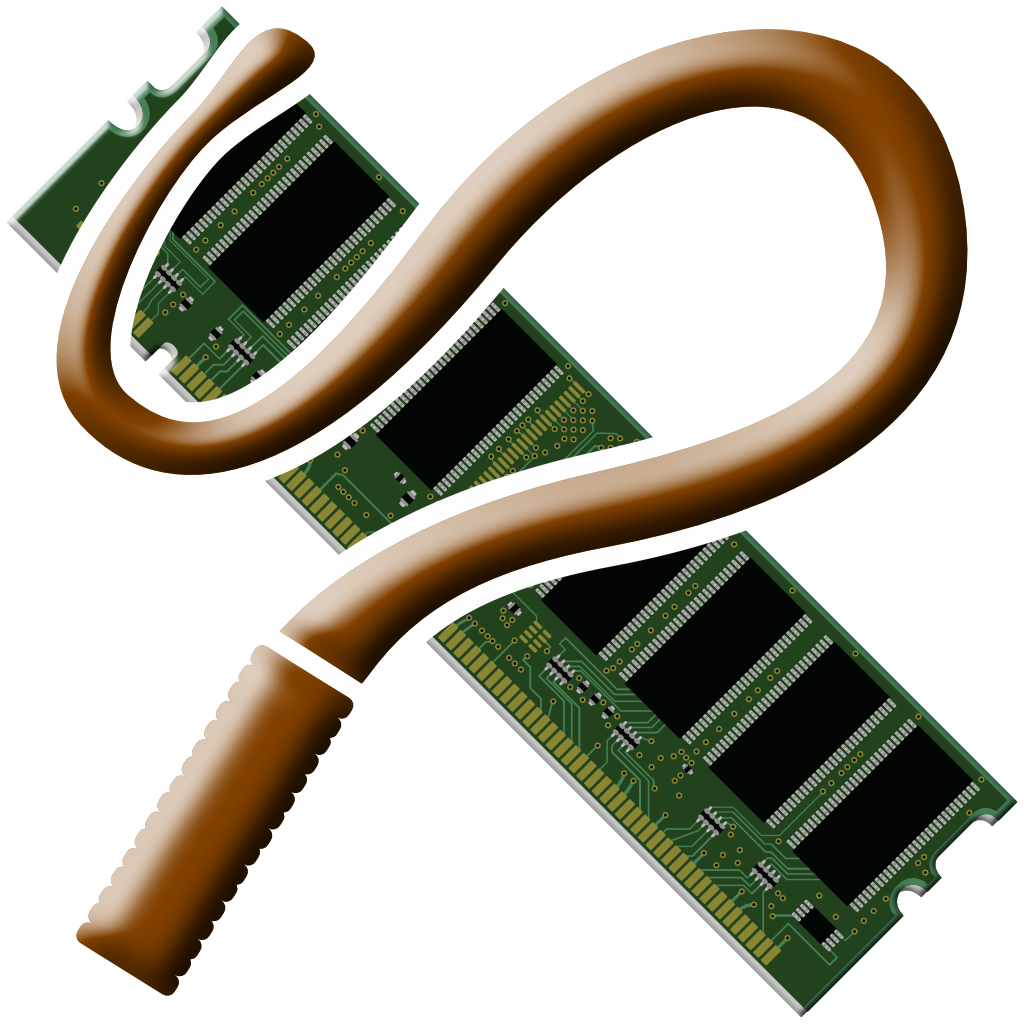
\includegraphics[width=128px]{../resources/Icon}\\
\MT\ User Manual
}
\author{Eric Henderson}
\date{Oct 1, 2014}
\maketitle

\clearpage
\tableofcontents
\clearpage
\section{Getting Started}

Most of the default preferences should be fine.  The main steps to get set up are to configure your notification preferences and configure the thresholds.  To open the preferences window, click on the \MT\ item in your menu bar and select ``Preferences''.

\subsection{Configuring Notification Preferences}
To configure notification preferences, open up the preferences window and go to the tab labeled ``Notifications''.  Here you can choose to use Notification Center (on OS X 10.8 Mountain Lion and up) or Growl, or to disable all notifications.  For Growl, you can make the notifications stay on the screen until you dismiss them.  You can also disable individual notifications.  \hyperref[notifications]{More on Notification Preferences}

\subsection{Configuring thresholds}
To configure freeing preferences, open up the preferences window and go to the tab labeled ``Freeing''.  Most of the default settings here are fine, but you should configure the thresholds. There are two different thresholds, one for regular freeing, and one for Memory Trimming.  Memory Trimming is a feature unique to \MT\ that will do a partial memory freeing at a higher threshold to reduce the frequency of full freeings.

\subsubsection*{Step 1 - Memory Trimming (optional, but recommended)}
If you want to enable Memory Trimming, you should set the trim threshold to a non-zero value (such as 1).  Memory Trimming is disabled by default, but it is recommended that you enable it.

\subsubsection*{Step 2 - Suggest Threshold}
The ``Suggest Threshold'' button will run a full freeing and then set the thresholds to be a certain percentage of the resulting free memory.  You may need to tweak these thresholds some, but ``Suggest Threshold'' will give you some good starting values.

\subsubsection*{Step 3 - Tweaking Thresholds}
It is possible that the ``Suggest Threshold'' functionality will give you thresholds that work really well.  However, in many cases, some tweaking is required.  If \MT\ is freeing memory too often, you will need to reduce the thresholds.  If it isn't keeping enough memory free, you will need to increase the thresholds.  There isn't a formula for the perfect thresholds, but with some trial and error, you can find values that work for you.

\subsection{Other preferences}
Besides the notification and freeing preferences, you may want to configure some of the preferences in the ``Display'' tab.  If your menu bar is low on space, you can set \MT\ to show only the icon or only the free memory.  You can also control the number of decimal places that are used for the free memory display and the frequency of updates to the menu bar item.\\
\\
Also, if you are low on space in your menu bar, you might find Bartender (\url{http://www.macbartender.com/}) quite useful.  It allows you to move menu bar items into a second, collapsible menu bar or hide them altogether.  It costs \$15 for a license, but I personally couldn't survive without it.

\clearpage
\section{Preferences}

\subsection{Notifications}
\label{notifications}
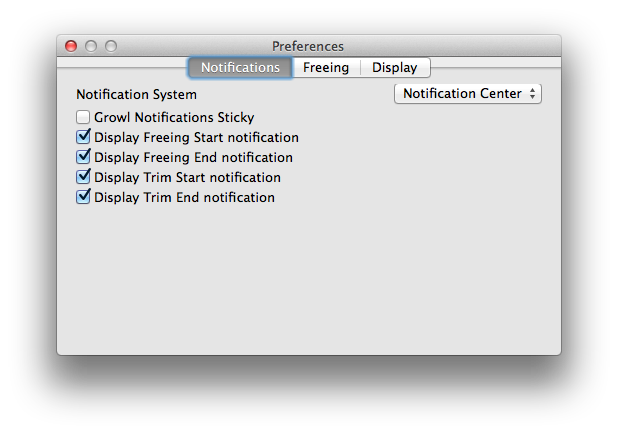
\includegraphics[width=400px]{notifications_tab}

\end{document}